% ------------------- chapter -------------------
%This is the extract from ICSBT article.
\chapter{Results and Discussions}
\label{ch:results}



% ------------------- paths to graphics -------------------

% change according to folder and file names
\ifpdf
    \graphicspath{{5_results/figures/}{5_results/figures/}
            {5_results/figures/}}
\else
    \graphicspath{{5_results/figures/EPS/}{5_results/figures/}}
\fi

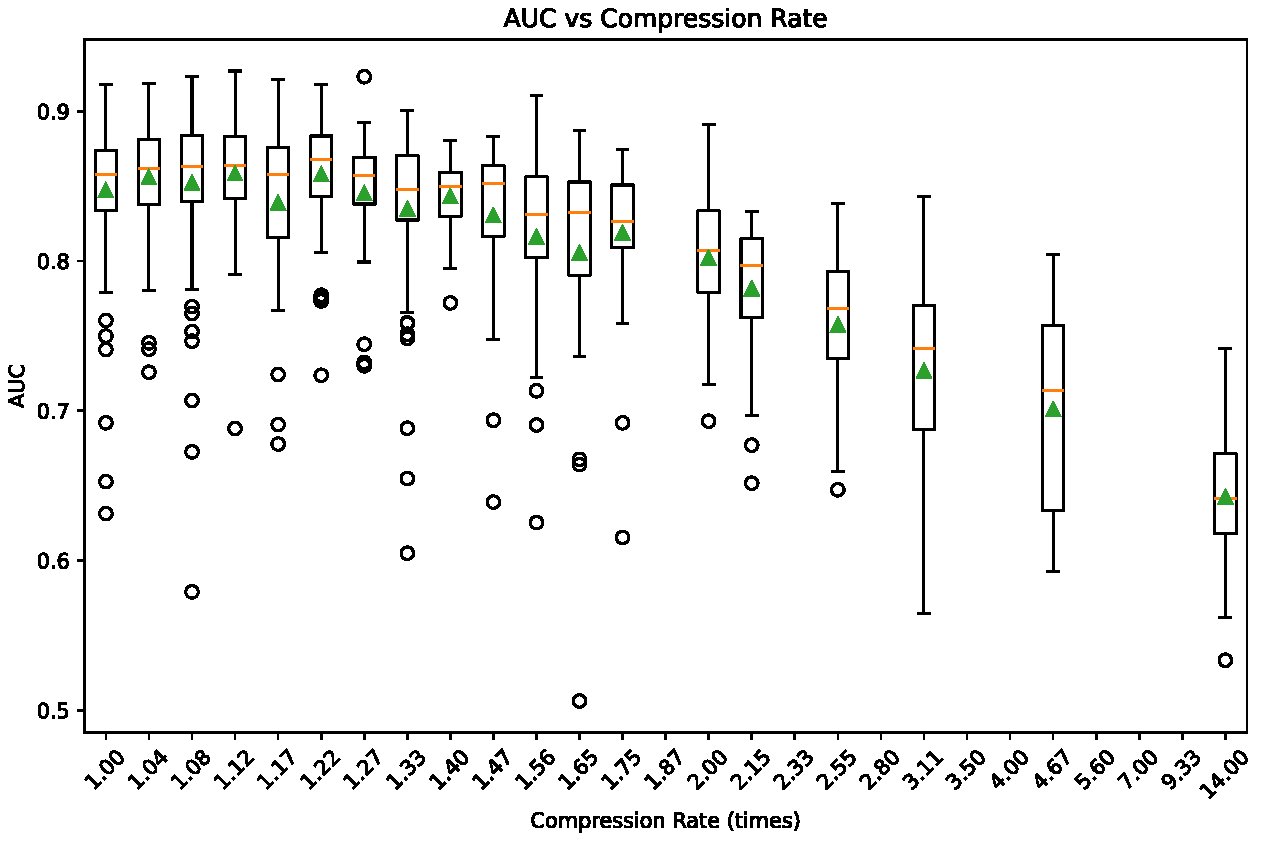
\includegraphics[width=1.2\textwidth]{search-compression-classify_model.pdf}



\section{Vanilla Autoencoder}
\label{sec:vanilla-ae}
For vanilla autoencoder, the concerns are mainly focused on the reconstruction quality of normal data and the ability to distinguish anomalies based on reconstruction errors.


\subsection{Reconstruction Quality on Normal Data}
To evaluate the reconstruction ability of the vanilla AE on normal operating conditions, we compute several standard metrics: mean average error (MAE), peak signal-to-noise ratio (PSNR), maximum reconstruction error, minimum reconstruction error, maximum min discrepancy and Wasserstein distance across time windows.

\begin{table}[h!]
\centering
\caption{Reconstruction metrics on normal validation data .}
\label{tab:rec_metrics_normal}
\begin{tabular}{lc}
\toprule
\textbf{Metric} & \textbf{Value} \\
\midrule
MAE                  & 0.0306 \\
PSNR [dB]            & 24.72 \\
Max error            & 0.1066 \\
Min error            & 0.0070 \\
Max--Min discrepancy & 0.0000 \\
Wasserstein distance & 0.0076 \\
\bottomrule
\end{tabular}
\end{table}

Overall, the reconstruction errors on normal validation data are low across all evaluated metrics, indicating that the vanilla AE learns to replicate healthy input signals with high fidelity. The mean absolute error (MAE) of $0.0306$ corresponds to a small deviation relative to the signal range, while the peak signal-to-noise ratio (PSNR) of $24.72$\,dB suggests a strong similarity between reconstructed and original signals. The maximum observed reconstruction error ($0.1066$) remains an order of magnitude smaller than typical anomaly-induced deviations, and the minimum error ($0.0070$) confirms that some time windows are reconstructed almost perfectly. The near-zero Max--Min discrepancy implies a consistent reconstruction quality across time windows, and the small Wasserstein distance ($0.0076$) shows that the overall error distribution closely matches that of the original data. These results confirm that the AE is capable of accurately modeling normal operating conditions.



\subsection{Normal vs. Abnormal Reconstruction}
For anomaly detection, the most straightforward approach is to use a static threshold on reconstruction error. For this study, ROC is first used to determine whether a significant difference exists in the reconstruction error between normal and abnormal samples.

\begin{table}[h!]
\centering
\caption{Feature-wise AUC for vanilla AE reconstruction error.}
\label{tab:vanilla_feat_auc}
\begin{tabular}{lc}
    \toprule
    \textbf{Feature} & \textbf{AUC} \\
    \midrule
    Power & 0.4449 \\
    Rotor speed & 0.5741 \\
    Wind speed & 0.4529 \\
    Air density & 0.6224 \\
    Temperature & 0.6163 \\
    Sin of Wind direction & 0.4499 \\
    Cos of Wind direction & 0.5460 \\
    \midrule
    \textbf{Overall} & \textbf{0.5036} \\
    \bottomrule
\end{tabular}
\end{table}

The overall AUC for the vanilla AE is close to 0.5, i.e., random performance, with feature-wise AUCs present in Table~\ref{tab:vanilla_feat_auc}.
The distribution of reconstruction errors for normal and abnormal validation samples is shown in Figure~\ref{fig:vanilla_norm_abnorm_roc}.

\begin{figure}[h!]
    \centering
    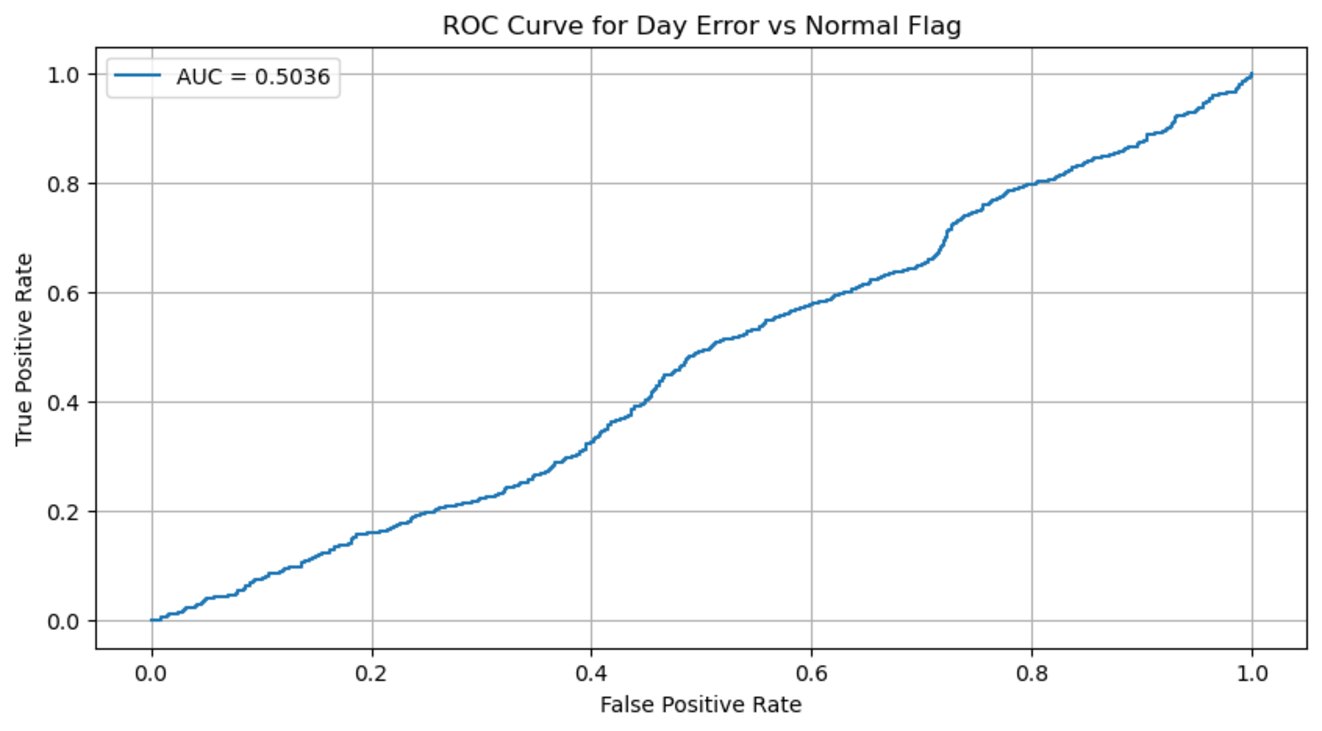
\includegraphics[width=\textwidth]{vanilla-roc.pdf}
    \caption{Vanilla AE ROC curve for normal vs. abnormal validation samples.}
    \label{fig:vanilla_norm_abnorm_roc}
\end{figure}


\begin{figure}[h!]
    \centering
    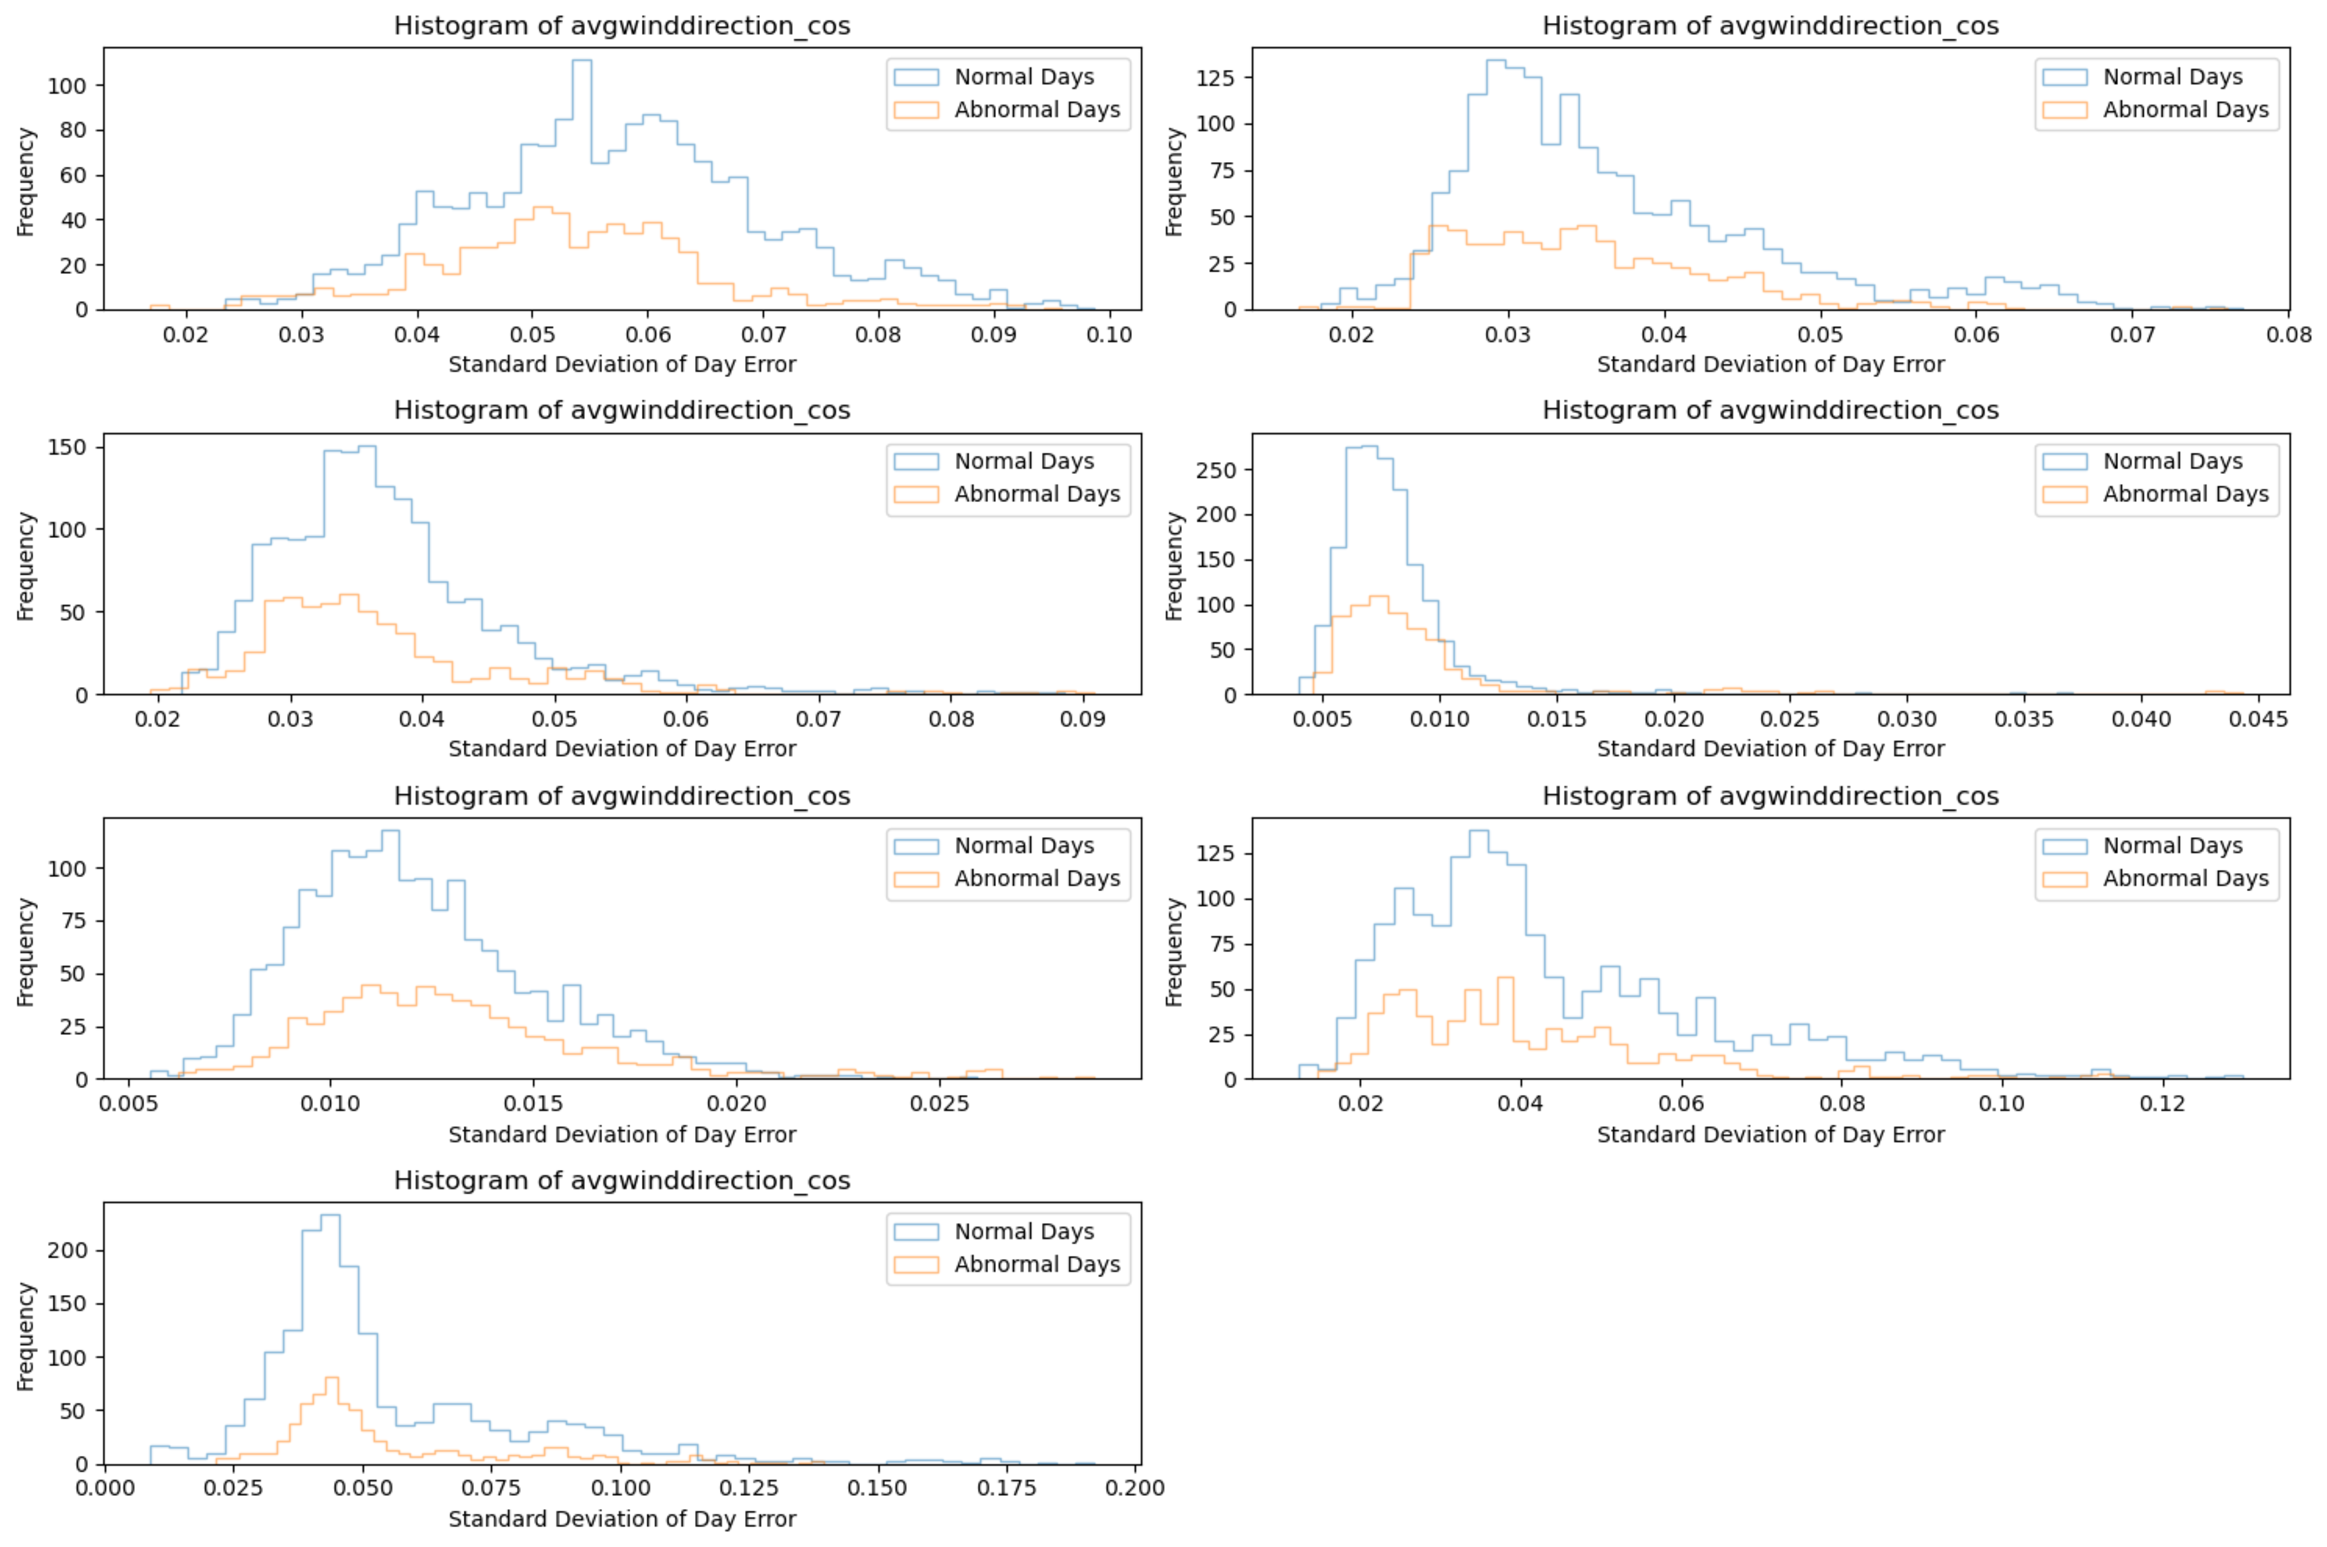
\includegraphics[width=\textwidth]{vanilla-reconst-hist.pdf}
    \caption{Vanilla AE reconstruction error (MSE) histogram for normal vs. abnormal validation samples.}
    \label{fig:vanilla_norm_abnorm_reconst_hist}
\end{figure}


Figure~\ref{fig:vanilla_norm_abnorm_reconst_hist}, Figure~\ref{fig:vanilla_norm_abnorm_roc} and Table~\ref{tab:vanilla_feat_auc} show that the vanilla AE is unable to create a linear separation between normal and abnormal samples based on reconstruction error. The AUC of $0.5036$ indicates that the model does not effectively distinguish between the two classes, as it is close to random guessing. The per-feature AUCs also suggest that some features provide a strong discrimination. It is easy to see that stable features such as air density and temperature have higher AUCs. These features are easier to reconstruct, thus, they are also more sensitive to anomalies.
However, they also did not provide enough information to achieve a meaningful separation overall.

\begin{figure}[h]
    \centering
    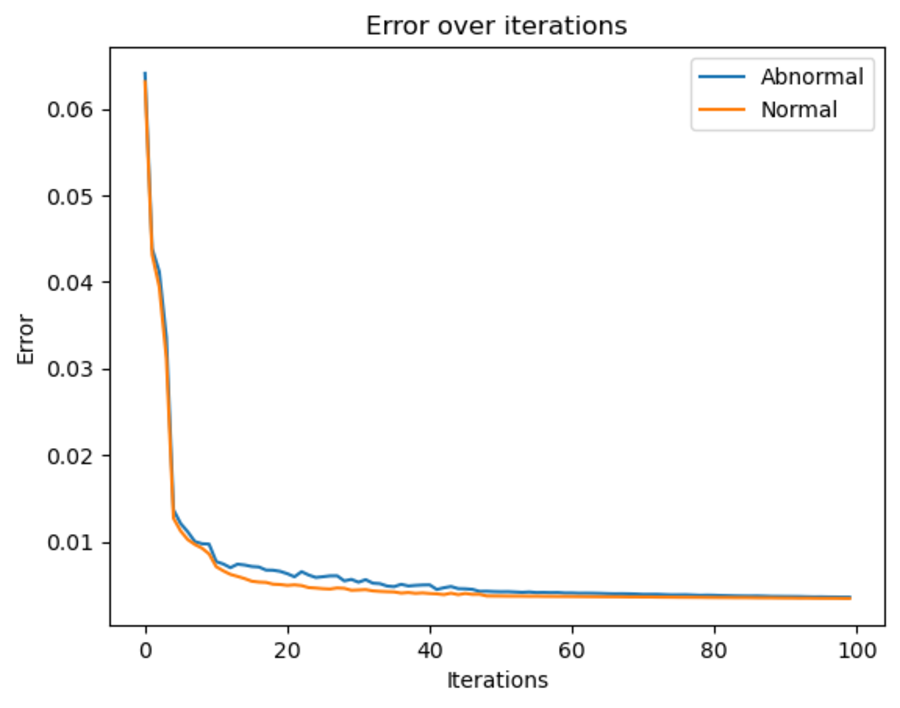
\includegraphics[width=0.85\textwidth]{vanilla-norm-abn-over-epoch.pdf}
    \caption{Reconstruction error (MSE) for normal and abnormal validation samples over training epochs.}
    \label{fig:vanilla_epoch_err}
\end{figure}

Given this poor separation, I further examined how reconstruction errors for normal and abnormal samples evolved throughout training (Figure~\ref{fig:vanilla_epoch_err}). Interestingly, the gap between the two classes is largest at around the 20th epoch, suggesting that the model initially learns to capture patterns specific to normal operating conditions while struggling to reconstruct abnormal signals. However, as training progresses, the reconstruction error for abnormal samples decreases to match that of normal samples. 
This convergence implies that the model gradually learns to represent both normal and abnormal patterns equally well, effectively "overfitting" to the anomalies present in the training set - the data that is nearly an abnormality. 
Consequently, the discriminative signal in reconstruction error is lost, explaining the near-random AUC observed in Table~\ref{tab:vanilla_feat_auc}.


This result suggests that either the difference in reconstruction error is highly non-linear and not captured by a simple threshold, or that the vanilla AE lacks the representational capacity for effective Normal Behavior Modeling in this dataset.




\subsection{Training Dynamics: Epoch-wise Behavior}
We monitor MSE over training epochs for both normal and abnormal validation sets.

\begin{figure}[h!]
    \centering
    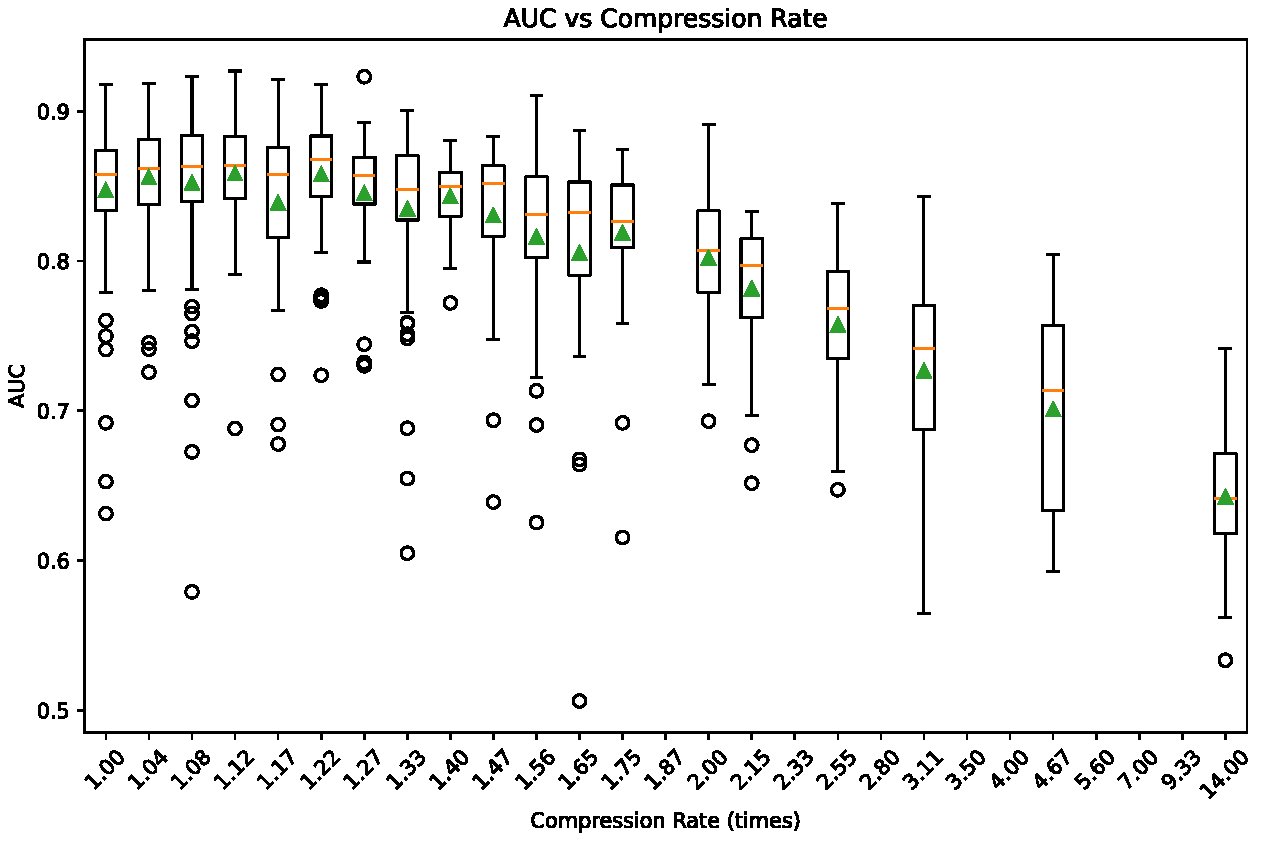
\includegraphics[width=0.85\textwidth]{search-compression-classify_model.pdf}
    \caption{Epoch-wise mean MSE for normal and abnormal validation sets. The difference $(\text{MSE}_{abn} - \text{MSE}_{norm})$ is also plotted.}
    \label{fig:vanilla_epoch_mse}
\end{figure}

As shown in Figure~\ref{fig:vanilla_epoch_mse}, \dots % interpretation

% ---------------------------------------------------------

\subsection{Aggregation Strategy Comparison}
Different aggregation strategies were applied to per-timestep errors for each window: mean, max, min, and $95^{\text{th}}$ percentile.

\begin{table}[h!]
\centering
\caption{Performance (AUC, F1, Precision, Recall) for different error aggregation strategies.}
\label{tab:agg_strategies}
\begin{tabular}{lcccc}
\toprule
\textbf{Aggregator} & \textbf{AUC} & \textbf{F1} & \textbf{Precision} & \textbf{Recall} \\
\midrule
Mean       & <value> & <value> & <value> & <value> \\
Max        & <value> & <value> & <value> & <value> \\
Min        & <value> & <value> & <value> & <value> \\
P95        & <value> & <value> & <value> & <value> \\
\bottomrule
\end{tabular}
\end{table}

\begin{figure}[h!]
    \centering
    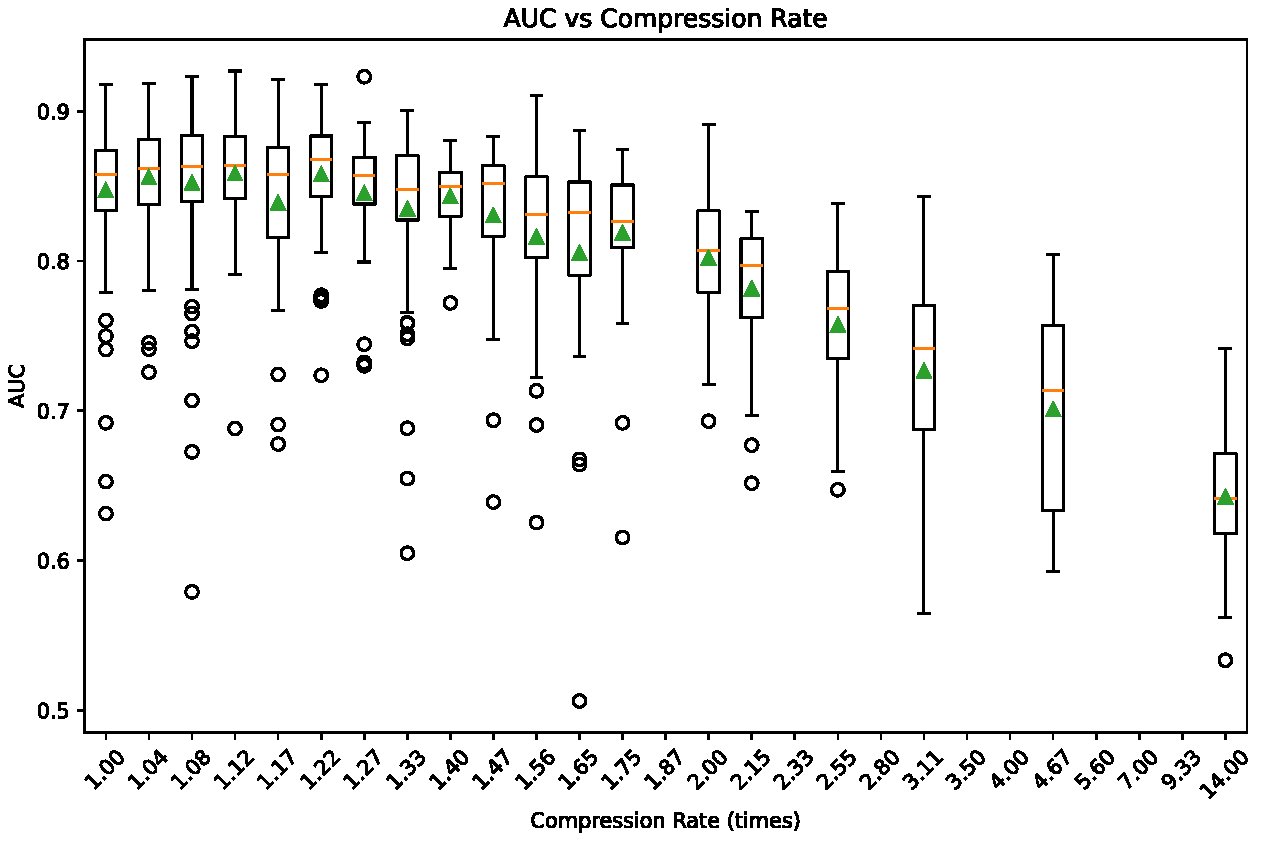
\includegraphics[width=0.85\textwidth]{search-compression-classify_model.pdf}
    \caption{ROC curves for different error aggregation strategies.}
    \label{fig:vanilla_roc_aggregators}
\end{figure}

% ---------------------------------------------------------

\subsection{Latent Size Sweep}
We evaluate the effect of latent size on reconstruction and detection performance.

\begin{table}[h!]
\centering
\caption{Effect of latent size on reconstruction and anomaly separability.}
\label{tab:latent_sweep}
\begin{tabular}{cccc}
\toprule
\textbf{Latent size} & \textbf{MSE$_{norm}$} & \textbf{MSE$_{abn}$} & \textbf{AUC} \\
\midrule
2   & <value> & <value> & <value> \\
4   & <value> & <value> & <value> \\
8   & <value> & <value> & <value> \\
16  & <value> & <value> & <value> \\
32  & <value> & <value> & <value> \\
64  & <value> & <value> & <value> \\
\bottomrule
\end{tabular}
\end{table}

\begin{figure}[h!]
    \centering
    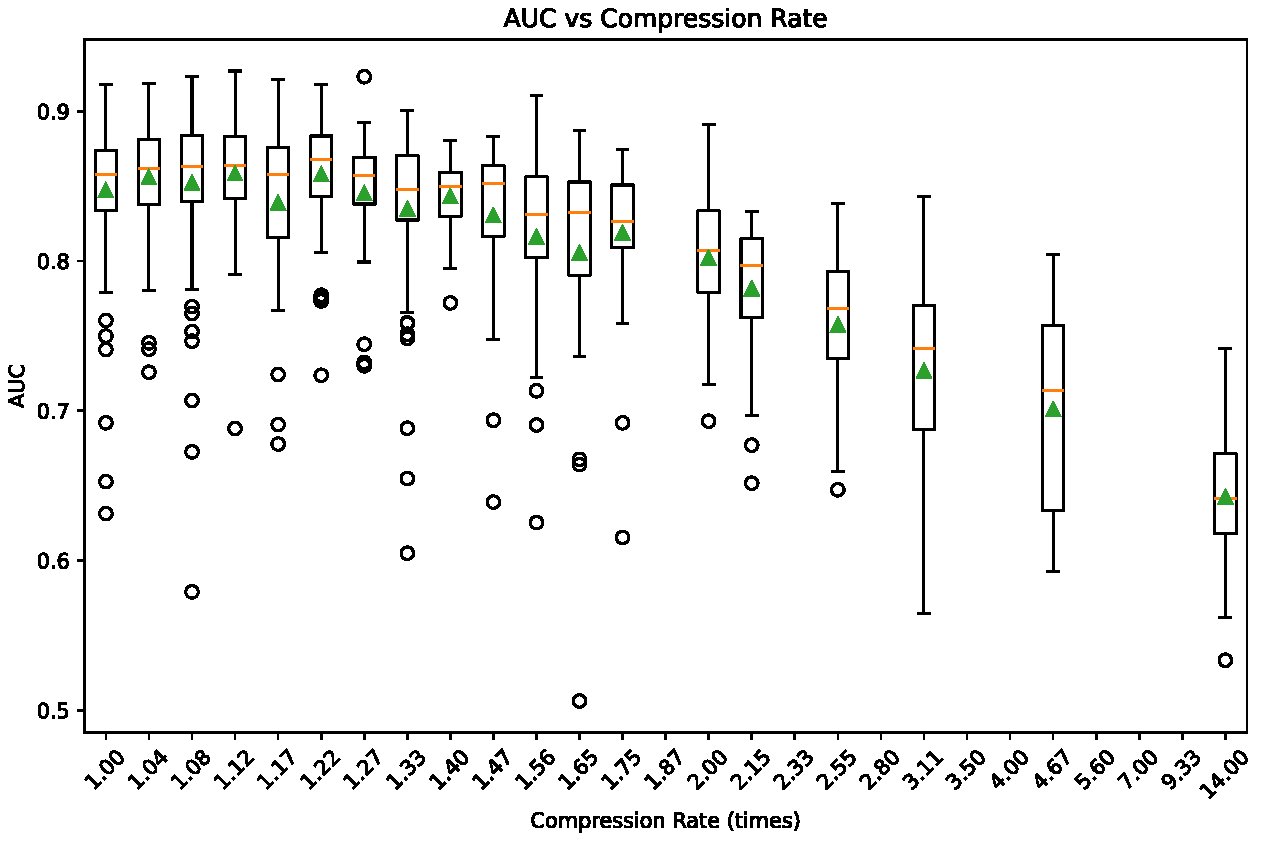
\includegraphics[width=0.85\textwidth]{search-compression-classify_model.pdf}
    \caption{AUC vs latent size.}
    \label{fig:vanilla_latent_auc}
\end{figure}

% ---------------------------------------------------------

\subsection{Per-feature Error Analysis}
Per-feature MSE was computed for normal and abnormal sets to identify which sensors contributed most to anomaly separability.

\begin{figure}[h!]
    \centering
    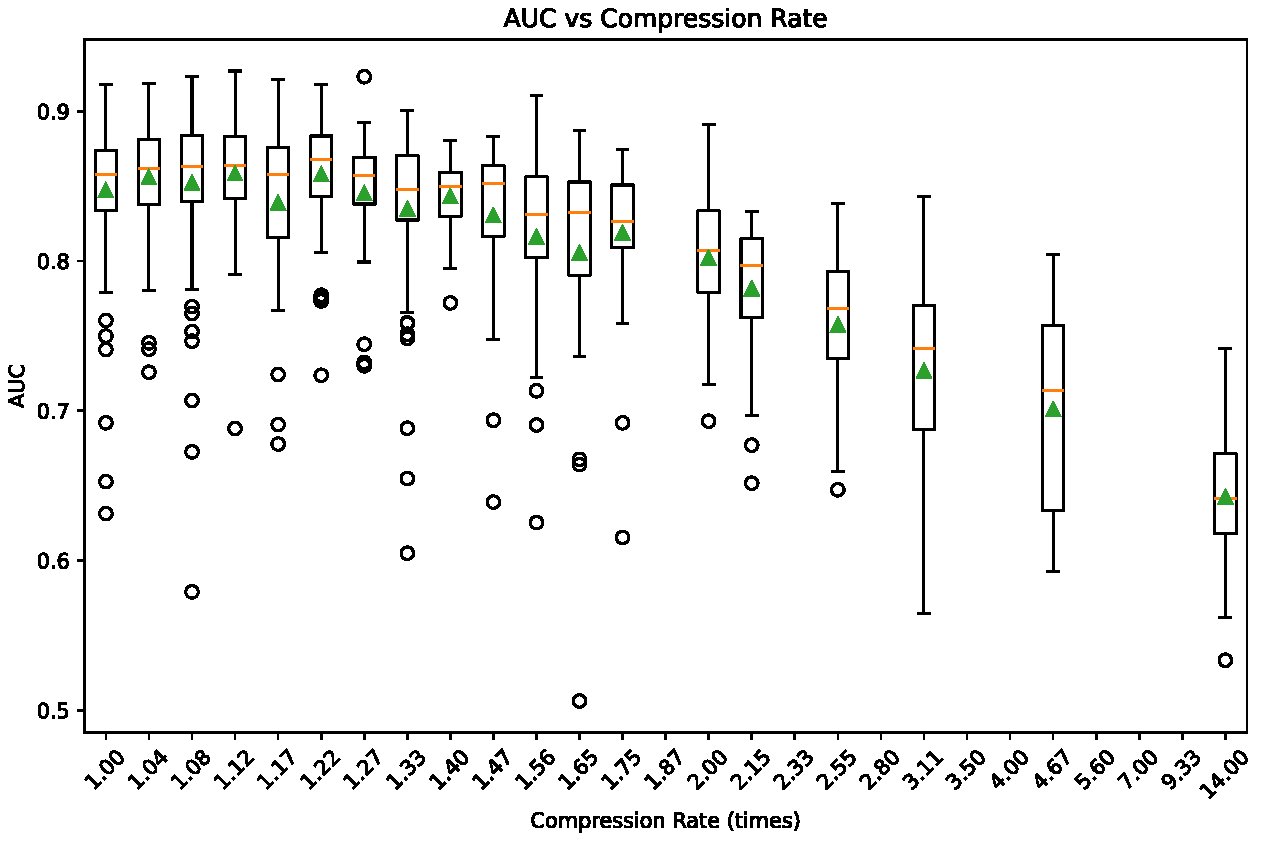
\includegraphics[width=0.9\textwidth]{search-compression-classify_model.pdf}
    \caption{Heatmap of per-feature MSE for normal and abnormal samples.}
    \label{fig:vanilla_feature_error_heatmap}
\end{figure}

\subsection{Summary}
In summary, the vanilla AE \dots % Your conclusion here.
